\documentclass[12pt, letterpaper, twoside]{article}
\usepackage[utf8]{inputenc}
\usepackage[margin=0.5in]{geometry}

\usepackage[T1]{fontenc}    % polish signs
\usepackage{multicol}

\usepackage{tikz}
\usepackage{pgfplots}
\usepgfplotslibrary{fillbetween}
\usetikzlibrary{patterns}
\pgfplotsset{compat=1.13}

\setlength{\parindent}{4em}
\setlength{\parskip}{1em}
\renewcommand{\baselinestretch}{1.5}

\begin{document}

\begin{center}
    $|\frac{x+1}{x-2}| \leq 2, x\neq2$
\end{center}

\begin{flushleft}
1. Z definicji wartości bezwzględnej.\\

\begin{multicols}{3}
$\frac{x+1}{x-2} \leq 2$\\
$\frac{x+1-2x+4}{x-2} \leq 0$\\
$\frac{-x+5}{x-2} \leq 0$\\
$(5-x)(x-2) \leq 0$\\

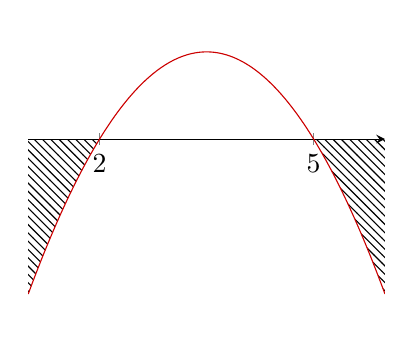
\begin{tikzpicture}
  \begin{axis}[
      axis x line=middle,
      axis y line=none,
      domain=1:6,
      xtick={2, 5},
      samples=1001,
      height=150pt,
    ]
    \addplot [red!80!black, name path=main] {(5-x)*(x-2)};
    
    % fills
    \path[name path=xaxis] (\pgfkeysvalueof{/pgfplots/xmin}, 0) -- (\pgfkeysvalueof{/pgfplots/xmax},0);
    \addplot[gray, pattern=north west lines] fill between[of=main and xaxis, soft clip={domain=1:2}];
    \addplot[gray, pattern=north west lines] fill between[of=main and xaxis, soft clip={domain=5:6}];
    
  \end{axis}
\end{tikzpicture}\\

$x\in(-\infty|2]\cup[5|\infty)$\\

\columnbreak
$\land$\\
\columnbreak
$\frac{x+1}{x-2} \geq -2$\\
$\frac{x+1+2x-4}{x-2} \geq 0$\\
$\frac{3x-3}{x-2} \geq 0$\\
$3(x-1)(x-2) \geq 0$\\

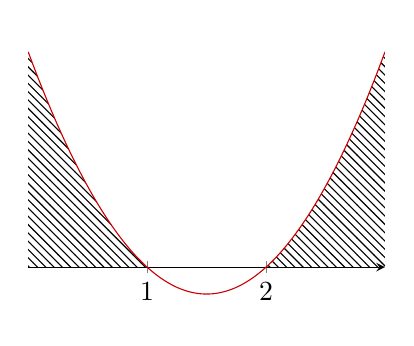
\begin{tikzpicture}
  \begin{axis}[
      axis x line=middle,
      axis y line=none,
      domain=0:3,
      xtick={1, 2},
      samples=1001,
      height=150pt,
    ]
    \addplot [red!80!black, name path=main] {(x-1)*(x-2)};
    
    % fills
    \path[name path=xaxis] (\pgfkeysvalueof{/pgfplots/xmin}, 0) -- (\pgfkeysvalueof{/pgfplots/xmax},0);
    \addplot[gray, pattern=north west lines] fill between[of=main and xaxis, soft clip={domain=0:1}];
    \addplot[gray, pattern=north west lines] fill between[of=main and xaxis, soft clip={domain=2:3}];
    
  \end{axis}
\end{tikzpicture}\\

$x\in(-\infty|1]\cup[2|\infty)$\\

\end{multicols}

\begin{center}
    $x\in(-\infty|1]\cup[5|\infty)$
\end{center}

\end{flushleft}

\begin{flushleft}
2. Mnożenie przez mianownik i użycie osi.\\

$|x+1| \leq 2|x-2|$

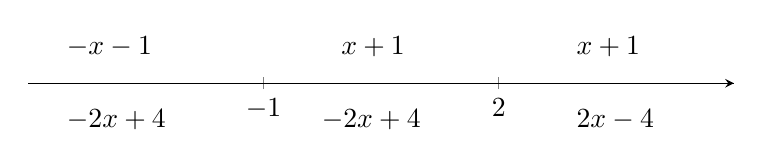
\begin{tikzpicture}
  \begin{axis}[
      axis x line=middle,
      axis y line=none,
      domain=-4:5,
      xtick={-1, 2},
      samples=1001,
      height=150pt,
      width=300pt,
    ]
    \addplot [black!80!black, name path=main] {0};
    
    % |x+1| (upper)
    \node[text width=3cm] at (-2,0.25) {$-x-1$};
    \node[text width=3cm] at (1.5,0.25) {$x+1$};
    \node[text width=3cm] at (4.5,0.25) {$x+1$};
    
    % 2|x-2| (lower)
    \node[text width=3cm] at (-2,-0.25) {$-2x+4$};
    \node[text width=3cm] at (1.25,-0.25) {$-2x+4$};
    \node[text width=3cm] at (4.5,-0.25) {$2x-4$};
    
  \end{axis}
\end{tikzpicture}\\

\begin{multicols}{3}
$x\in(-\infty|-1)$\\
$-x-1\leq-2x+4$\\
$x\leq5$\\
$x\in(-\infty|-1)$\\
\columnbreak
$x\in[-1|2)$\\
$x+1\leq-2x+4$\\
$3x\leq3$\\
$x\leq1$\\
$x\in[-1|1]$\\
\columnbreak
$x\in(2|\infty)$\\
$x+1\leq2x-4$\\
$x\geq5$\\
$x\in[5|\infty)$\\
\end{multicols}

\begin{center}
    $x\in(-\infty|1]\cup[5|\infty)$\\
\end{center}

\end{flushleft}

\pagebreak

\begin{flushleft}
3. Analiza wykresu.\\

\begin{tikzpicture}
  \begin{axis}[
      axis x line=middle,
      axis y line=middle,
      domain=-4:6,
      restrict y to domain=-10:6,
      xtick={2},
      ytick={1, 2},
      samples=1001,
      height=150pt,
    ]
    \addplot [red!80!black, name path=main] {abs((x+1)/(x-2))};
    
    % asymptotes
    \draw [dashed] (2,-1) -- (2,6);
    \draw [dashed] (-4,1) -- (6,1);
    
    \draw [dashed] (-4,2) -- (6,2);
    
  \end{axis}
\end{tikzpicture}\\

$|\frac{x+1}{x-2}|=2$\\
\begin{multicols}{3}
$\frac{x+1}{x-2}=2$\\
$x+1-2x+4=0$\\
$-x+5=0$\\
$x=5$\\
\columnbreak
$\lor$\\
\columnbreak
$\frac{x+1}{x-2}=-2$\\
$x+1+2x-4=0$\\
$3x-3=0$\\
$x=1$\\
\end{multicols}

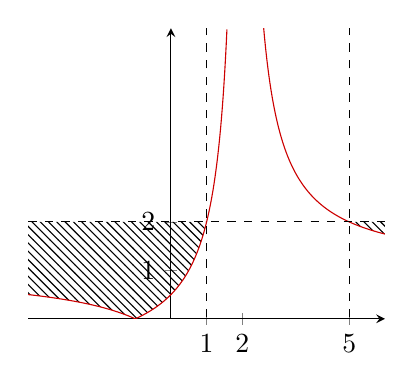
\begin{tikzpicture}
  \begin{axis}[
      axis x line=middle,
      axis y line=middle,
      domain=-4:6,
      restrict y to domain=-10:6,
      xtick={1,2,5},
      ytick={1,2},
      samples=1001,
      height=150pt,
    ]
    \addplot [red!80!black, name path=main] {abs((x+1)/(x-2))};
    
    \draw [dashed] (1,-1) -- (1,6);
    \draw [dashed] (5,-1) -- (5,6);
    
    \draw [dashed] (-4,2) -- (6,2);
    
    % fills
    \path[name path=xaxis] (\pgfkeysvalueof{/pgfplots/xmin}, 2) -- (\pgfkeysvalueof{/pgfplots/xmax},2);
    \addplot[gray, pattern=north west lines] fill between[of=main and xaxis, soft clip={domain=-4:1}];
    \addplot[gray, pattern=north west lines] fill between[of=main and xaxis, soft clip={domain=5:6}];
    
  \end{axis}
\end{tikzpicture}\\

$x\in(-\infty|1]\cup[5|\infty)$\\

\end{flushleft}

\begin{flushleft}
4. Mnożenie przez mianownik i analiza dwóch wykresów.\\

$|x+1|\leq2|x-2|$\\

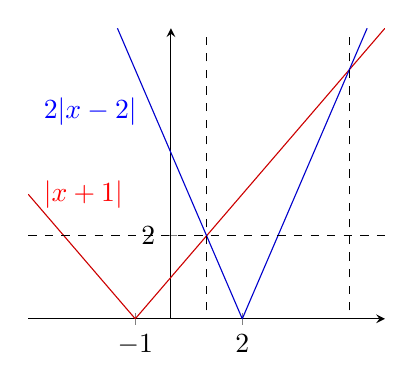
\begin{tikzpicture}
  \begin{axis}[
      axis x line=middle,
      axis y line=middle,
      domain=-4:6,
      restrict y to domain=-10:7,
      xtick={-1, 2},
      ytick={2},
      samples=1001,
      height=150pt,
    ]
    \addplot [red!80!black, name path=main1] {abs(x+1)};
    \addplot [blue!80!black, name path=main2] {2*abs(x-2)};
    
    \draw [dashed] (-4,2) -- (6,2);
    
    % labels
    \node[text width=3cm, color=red] at (-0.25,3) {$|x+1|$};
    \node[text width=3cm, color=blue] at (-0.25,5) {$2|x-2|$};
    
    \draw [dashed] (1,-1) -- (1,7);
    \draw [dashed] (5,-1) -- (5,7);
    
  \end{axis}
\end{tikzpicture}\\

$|x+1|=2|x-2|$\\

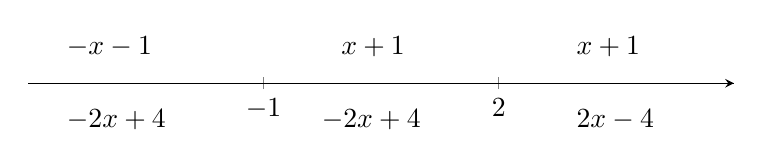
\begin{tikzpicture}
  \begin{axis}[
      axis x line=middle,
      axis y line=none,
      domain=-4:5,
      xtick={-1, 2},
      samples=1001,
      height=150pt,
      width=300pt,
    ]
    \addplot [black!80!black, name path=main] {0};
    
    % |x+1| (upper)
    \node[text width=3cm] at (-2,0.25) {$-x-1$};
    \node[text width=3cm] at (1.5,0.25) {$x+1$};
    \node[text width=3cm] at (4.5,0.25) {$x+1$};
    
    % 2|x-2| (lower)
    \node[text width=3cm] at (-2,-0.25) {$-2x+4$};
    \node[text width=3cm] at (1.25,-0.25) {$-2x+4$};
    \node[text width=3cm] at (4.5,-0.25) {$2x-4$};
    
  \end{axis}
\end{tikzpicture}\\

\begin{multicols}{3}
$x\in(-\infty|-1)$\\
$-x-1=-2x+4$\\
$x=5$\\
$x\in\emptyset$\\
\columnbreak
$x\in[-1|2)$\\
$x+1=-2x+4$\\
$3x=3$\\
$x=1$\\
\columnbreak
$x\in(2|\infty)$\\
$x+1=2x-4$\\
$x=5$\\
\end{multicols}

\begin{center}
    $x=1\lor x=5$\\
\end{center}

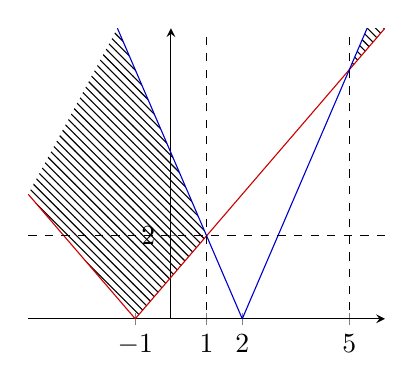
\begin{tikzpicture}
  \begin{axis}[
      axis x line=middle,
      axis y line=middle,
      domain=-4:6,
      restrict y to domain=-10:7,
      xtick={-1, 1, 2, 5},
      ytick={2},
      samples=1001,
      height=150pt,
    ]
    \addplot [red!80!black, name path=main1] {abs(x+1)};
    \addplot [blue!80!black, name path=main2] {2*abs(x-2)};
    
    \draw [dashed] (-4,2) -- (6,2);
    
    \draw [dashed] (1,-1) -- (1,7);
    \draw [dashed] (5,-1) -- (5,7);
    
    % fills
    \addplot[gray, pattern=north west lines] fill between[of=main1 and main2, soft clip={domain=-4:1}];
    \addplot[gray, pattern=north west lines] fill between[of=main1 and main2, soft clip={domain=5:6}];
    
  \end{axis}
\end{tikzpicture}\\

$x\in(-\infty|1]\cup[5|\infty)$\\

\end{flushleft}

\begin{flushleft}
5. Rozbicie licznika do łatwiejszej do obliczenia postaci.\\
$|\frac{x+1}{x-2}|=|\frac{x-2+3}{x-2}|=|1+\frac{3}{x-2}|$\\

\begin{multicols}{3}
$1+\frac{3}{x-2} \leq 2$\\
$\frac{3-x+2}{x-2} \leq 0$\\
$\frac{5-x}{x-2} \leq 0$\\
$(5-x)(x-2) \leq 0$\\

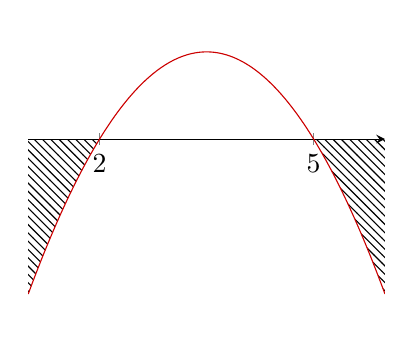
\begin{tikzpicture}
  \begin{axis}[
      axis x line=middle,
      axis y line=none,
      domain=1:6,
      xtick={2, 5},
      samples=1001,
      height=150pt,
    ]
    \addplot [red!80!black, name path=main] {(5-x)*(x-2)};
    
    % fills
    \path[name path=xaxis] (\pgfkeysvalueof{/pgfplots/xmin}, 0) -- (\pgfkeysvalueof{/pgfplots/xmax},0);
    \addplot[gray, pattern=north west lines] fill between[of=main and xaxis, soft clip={domain=1:2}];
    \addplot[gray, pattern=north west lines] fill between[of=main and xaxis, soft clip={domain=5:6}];
    
  \end{axis}
\end{tikzpicture}\\

$x\in(-\infty|2]\cup[5|\infty)$\\

\columnbreak
$\land$\\
\columnbreak
$1+\frac{3}{x-2} \leq -2$\\
$\frac{3+3x-6}{x-2} \leq 0$\\
$\frac{3x-3}{x-2} \leq 0$\\
$3(x-1)(x-2) \leq 0$\\


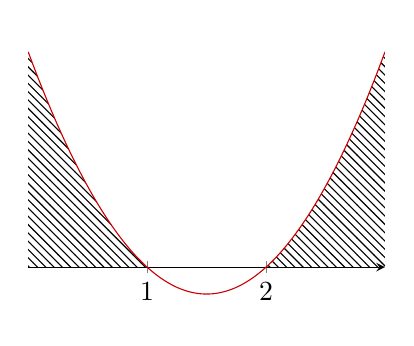
\begin{tikzpicture}
  \begin{axis}[
      axis x line=middle,
      axis y line=none,
      domain=0:3,
      xtick={1, 2},
      samples=1001,
      height=150pt,
    ]
    \addplot [red!80!black, name path=main] {(x-1)*(x-2)};
    
    % fills
    \path[name path=xaxis] (\pgfkeysvalueof{/pgfplots/xmin}, 0) -- (\pgfkeysvalueof{/pgfplots/xmax},0);
    \addplot[gray, pattern=north west lines] fill between[of=main and xaxis, soft clip={domain=0:1}];
    \addplot[gray, pattern=north west lines] fill between[of=main and xaxis, soft clip={domain=2:3}];
    
  \end{axis}
\end{tikzpicture}\\

$x\in(-\infty|1]\cup[2|\infty)$\\

\end{multicols}

\begin{center}
    $x\in(-\infty|1]\cup[5|\infty)$
\end{center}

\end{flushleft}

\end{document}

